\documentclass[11pt]{article}
\usepackage[margin=1in]{geometry}
\usepackage{amsmath, amssymb}
\usepackage{graphicx}
\usepackage{booktabs}
\usepackage{hyperref}
\usepackage{listings}
\usepackage{xcolor}
\usepackage{enumitem}
\usepackage{caption}
\usepackage{subcaption}
\usepackage{parskip}

\lstset{
  language=Python,
  basicstyle=\ttfamily\small,
  keywordstyle=\color{blue},
  commentstyle=\color{gray},
  stringstyle=\color{orange},
  showstringspaces=false,
  frame=single,
  breaklines=true,
}

\title{\textbf{CS265 MLSys Project: Midway Check-in Report}\\
       \large Phase 1: Computational Graph Profiler}
\author{[Your Name]}
\date{Spring 2025}

\begin{document}
\maketitle

% ============================================================
\section{Introduction}
% ============================================================

This milestone implements the first phase of an activation checkpointing
system for deep neural network training in PyTorch.
Activation checkpointing is a memory optimization that reduces peak GPU
memory consumption by discarding a subset of intermediate tensors
(activations) after the forward pass and recomputing them on demand
during the backward pass.
To decide which activations to discard, we need a profiler that
characterizes the computational cost and memory footprint of every
operation in a full training iteration.

In Phase~1, we build a \emph{computational graph profiler} on top of
PyTorch's \texttt{torch.fx} framework.
The profiler captures the full training step (forward pass, loss,
backward pass, and optimizer update) as a single flat
\texttt{fx.GraphModule} and performs static analysis to classify each
node by its role: model parameter, activation, gradient, optimizer
state, or input batch.
It then identifies which nodes are activations and records their
lifetime boundaries in the graph (last use in forward, first use in
backward).
At runtime it measures per-node GPU execution time using CUDA Events
and tracks memory allocation deltas.
We validate the profiler on a simple linear model, then apply it to
ResNet18, ResNet50, and a Transformer, collecting profiling statistics
and peak-memory breakdowns across batch sizes.

% ============================================================
\section{Problems Tackled}
% ============================================================

\begin{itemize}[leftmargin=*]

  \item \textbf{[Graph Capture]}
    We need to capture the entire training step (forward, backward,
    and optimizer) as a single inspectable static graph so that all
    operations and data dependencies are available for profiling and
    later graph rewriting.

  \item \textbf{[Forward/Backward Boundary Detection]}
    Within the combined graph we need to reliably identify which nodes
    belong to the forward pass and which to the backward pass, in order
    to correctly classify activation nodes and measure their idle
    lifetimes in GPU memory.

  \item \textbf{[Node Classification]}
    Nodes in the graph may represent model parameters, input batches,
    optimizer states, gradient tensors, or activation tensors, yet they
    are all represented identically as \texttt{fx.Node} objects.
    We need a rule-based classifier to assign each node a semantic type
    and produce a meaningful memory breakdown.

  \item \textbf{[Activation Lifetime and Runtime Profiling]}
    For each activation, Phase~2 needs its last use in the forward pass,
    its first use in the backward pass, its size in bytes, and its
    recomputation cost in milliseconds.
    Collecting this accurately requires care because CUDA kernels execute
    asynchronously.

\end{itemize}

% ============================================================
\section{Technical Description}
% ============================================================

% -------------------------------------------------------
\subsection{Graph Capture}
% -------------------------------------------------------

\paragraph{a) Problem framing.}
PyTorch's standard training loop uses dynamic autograd: the backward
graph is built at runtime during the forward pass and discarded after
each iteration.
This prevents any static inspection of backward operations or the
optimizer update.
Without a static representation of the full iteration, we cannot profile
individual operations, analyze tensor lifetimes, or inject recomputation
subgraphs (needed in Phase~3).

\paragraph{b) High-level solution.}
We use \texttt{make\_fx} from \texttt{torch.fx.experimental.proxy\_tensor}
to trace a stateless version of the training step.
\texttt{make\_fx} executes the function with fake (symbolic) tensors and
records every ATen-level operation into a flat \texttt{fx.GraphModule}.
Because both the forward and backward computations are recorded in the
same tracing call, the resulting graph contains all three phases in a
single node sequence.

\paragraph{c) Deeper details.}
Three preparatory steps make the trace possible.
\begin{enumerate}
  \item \textbf{Stateless re-parametrization.}
    Model parameters and optimizer states are lifted out of the module
    and optimizer objects and passed as explicit function arguments.
    This forces \texttt{make\_fx} to expose the optimizer update as
    ordinary graph nodes rather than side effects on Python objects.
  \item \textbf{Separator injection.}
    A custom no-op, \texttt{SEPFunction}, is applied to the scalar loss
    at the end of the forward pass.
    It registers two ATen operators, \texttt{separator.sep} and
    \texttt{separator.sep\_backward}, which appear as nodes in the graph
    and serve as unambiguous markers of the forward/backward boundary.
  \item \textbf{Decomposition.}
    In-place \texttt{foreach} optimizer kernels (e.g.,
    \texttt{\_foreach\_add\_}) are decomposed into out-of-place
    operations followed by \texttt{copy\_} nodes, making the graph
    fully functional and easier to analyze.
\end{enumerate}

% -------------------------------------------------------
\subsection{Forward/Backward Boundary Detection}
% -------------------------------------------------------

\paragraph{a) Problem framing.}
The combined graph contains hundreds to thousands of nodes from all
three phases.
An activation is defined as a non-placeholder tensor created in the
forward pass and consumed in the backward pass.
Without knowing which nodes belong to which phase, this definition
cannot be evaluated.

\paragraph{b) High-level solution.}
We scan the graph's node list (which is already in topological order)
once to locate two indices:
\begin{itemize}
  \item \texttt{sep\_idx}: position of the \texttt{separator.sep} node
    (end of forward pass)
  \item \texttt{sep\_bwd\_idx}: position of the
    \texttt{separator.sep\_backward} node (start of backward pass)
\end{itemize}
All nodes at positions below \texttt{sep\_idx} are \emph{forward nodes};
all nodes at positions above \texttt{sep\_bwd\_idx} are
\emph{backward/optimizer nodes}.

\paragraph{c) Deeper details.}
The partition runs in $\mathcal{O}(N)$ time and is stored as two Python
sets for $\mathcal{O}(1)$ membership queries during classification.
The small region between the two sentinels (containing the loss value
and its backward initiation) is classified as \texttt{OTHER} and
excluded from both regions.
Listing~\ref{lst:boundary} shows the core logic.

\begin{lstlisting}[caption={Boundary detection (simplified)},
                   label={lst:boundary}]
for i, node in enumerate(nodes):
    if node.target is torch.ops.separator.sep.default:
        sep_idx = i
    elif node.target is torch.ops.separator.sep_backward.default:
        sep_bwd_idx = i

forward_nodes  = {n for n in nodes if idx[n] < sep_idx}
backward_nodes = {n for n in nodes if idx[n] > sep_bwd_idx}
\end{lstlisting}

% -------------------------------------------------------
\subsection{Node Classification}
% -------------------------------------------------------

\paragraph{a) Problem framing.}
A node may represent a model weight, an activation, a gradient, an
optimizer state (e.g., Adam first/second moment), or the input batch,
yet all of these appear as either \texttt{placeholder} or
\texttt{call\_function} nodes with no explicit label.
Assigning correct types is necessary to produce a meaningful memory
breakdown and to identify activation candidates for checkpointing.

\paragraph{b) High-level solution.}
We classify nodes using a two-step heuristic.
\begin{enumerate}
  \item \textbf{Placeholder classification.}
    We locate the final weight-update kernel (\texttt{\_foreach\_addcdiv}
    for \texttt{foreach=True} Adam).
    Its first argument group are the model \textbf{parameters}; other
    placeholder nodes with users in the backward region are
    \textbf{optimizer states}.
    The remaining placeholders are the input \textbf{batch}.
  \item \textbf{Non-placeholder classification.}
    A \texttt{call\_function} node in the forward region whose user set
    intersects the backward node set is an \textbf{activation}
    (\texttt{ACT}).
    All other non-placeholder nodes in the backward region are
    \textbf{gradients} (\texttt{GRAD}).
\end{enumerate}

\paragraph{c) Deeper details.}
Table~\ref{tab:nodetypes} summarizes all classification rules.
The full pass runs in $\mathcal{O}(N \cdot D)$ time, where $D$ is the
average out-degree of a node, bounded by the number of backward users
per activation.

\begin{table}[h]
\centering
\caption{Node type classification rules}
\label{tab:nodetypes}
\begin{tabular}{lll}
\toprule
\textbf{NodeType} & \textbf{Op} & \textbf{Rule} \\
\midrule
PARAM  & placeholder     & First arg group of the optimizer update kernel \\
OPT    & placeholder     & Other placeholders with backward-region users \\
INPUT  & placeholder     & All remaining placeholders \\
ACT    & call\_function  & Forward region; at least one user in backward region \\
GRAD   & call\_function  & Backward/optimizer region \\
OTHER  & any             & Sentinel nodes, loss, output, getitem \\
\bottomrule
\end{tabular}
\end{table}

% -------------------------------------------------------
\subsection{Activation Lifetime and Runtime Profiling}
% -------------------------------------------------------

\paragraph{a) Problem framing.}
Phase~2 needs four values per activation: its last use in forward, its
first use in backward, its size in bytes, and its recomputation cost in
milliseconds.
The first two determine how long the tensor sits idle in GPU memory
before it is needed again; the latter two determine whether discarding
and recomputing it saves more memory than it costs in time.
Accurate per-node timing is non-trivial because CUDA kernels execute
asynchronously relative to the Python host.

\paragraph{b) High-level solution.}
\textbf{Lifetimes} are computed purely from graph structure:
\begin{align*}
  \texttt{last\_fwd\_use}(a)  &= \arg\max_{u \,\in\, \text{users}(a)\,\cap\, F}\ \text{idx}(u) \\
  \texttt{first\_bwd\_use}(a) &= \arg\min_{u \,\in\, \text{users}(a)\,\cap\, B}\ \text{idx}(u)
\end{align*}
where $F$ and $B$ are the forward and backward node sets.

\textbf{Runtime} is measured by overriding \texttt{fx.Interpreter.run\_node}
to wrap each node execution with \texttt{torch.cuda.Event} objects.
GPU memory is sampled before and after via
\texttt{torch.cuda.memory\_allocated()}.
We run 2 warm-up iterations (discarded) then 3 measurement iterations;
all values are averaged by \texttt{aggregate\_stats()}.

\paragraph{c) Deeper details.}
Listing~\ref{lst:runnode} shows the per-node measurement code.
\texttt{torch.cuda.synchronize()} is called after \texttt{end.record()}
to block the CPU until all pending CUDA work completes, ensuring both
the elapsed time and the memory sample are accurate.
Without synchronization, \texttt{elapsed\_time} would still block
eventually, but the memory reading could be taken before the kernel
has actually allocated its output.

\begin{lstlisting}[caption={Per-node timing in \texttt{run\_node}},
                   label={lst:runnode}]
def run_node(self, n):
    start = torch.cuda.Event(enable_timing=True)
    end   = torch.cuda.Event(enable_timing=True)
    mem_before = torch.cuda.memory_allocated()
    start.record()
    result = super().run_node(n)
    end.record()
    torch.cuda.synchronize()
    self._runtimes[n].append(start.elapsed_time(end))        # ms
    self._mem_delta[n].append(
        torch.cuda.memory_allocated() - mem_before)          # bytes
    return result
\end{lstlisting}

To build the memory breakdown chart in Figure~\ref{fig:memory}, we
simulate the memory timeline after profiling: we walk nodes in order,
add a tensor's byte size when its producer executes, and subtract it
when its last user executes.
At each step we record the running total per category and take the
per-category maximum as the peak.

% ============================================================
\section{Experimental Results}
% ============================================================

\subsection{Per-model Profiling Statistics}

Table~\ref{tab:profresults} shows the aggregate profiling results for
the three benchmark models at their default batch sizes.
The backward pass takes roughly $4.5\times$ to $5\times$ longer than
the forward pass across all models, consistent with the theoretical
expectation that backward must compute both input and weight gradients
for each layer.
Activation memory for the ResNets (approximately 350~MB) is much larger
than for the Transformer (19~MB).
This is because ResNet feature maps scale with both spatial resolution
and batch size, whereas most Transformer intermediate tensors are
\texttt{view} operations that share storage with their inputs and do
not allocate fresh GPU memory.

\begin{table}[h]
\centering
\caption{Profiling summary (3 iterations, 2 warm-up, default batch sizes)}
\label{tab:profresults}
\begin{tabular}{lrrrr}
\toprule
\textbf{Model} & \textbf{Batch size} & \textbf{Fwd (ms)} &
\textbf{Bwd (ms)} & \textbf{Activation mem (MB)} \\
\midrule
ResNet18     & 16 & 21.0  & 104.2 & 347 \\
ResNet50     & 4  & 51.5  & 238.1 & 350 \\
Transformer  & 4  & 34.2  & 163.6 &  19 \\
\bottomrule
\end{tabular}
\end{table}

\subsection{Static Analysis: Activation Lifetimes}

On the DummyModel (10-layer linear network, batch 1000, dim 100), the
profiler found 19 activation nodes: 10 \texttt{relu} outputs (0.40~MB
each) and 9 transposed weight matrices \texttt{t\_*} (0.04~MB each),
totaling 4.36~MB.
The first layer's activation (\texttt{relu}) has its last forward use
at \texttt{addmm\_1} but is not needed again until \texttt{mm\_17},
near the very end of the backward pass.
This confirms the key property that earlier-layer activations sit idle
in memory the longest, which is exactly what activation checkpointing
targets.

\subsection{Peak Memory vs.\ Batch Size}

Figure~\ref{fig:memory} shows the stacked peak memory breakdown across
batch sizes for each model.
Activations (orange bars) are the dominant consumer and grow roughly
linearly with batch size.
Parameters and optimizer states stay flat across batch sizes, as
expected, since they depend only on model size.
These results confirm that activations are the right target for memory
reduction.

\begin{figure}[h]
  \centering
  \begin{subfigure}[b]{0.48\textwidth}
    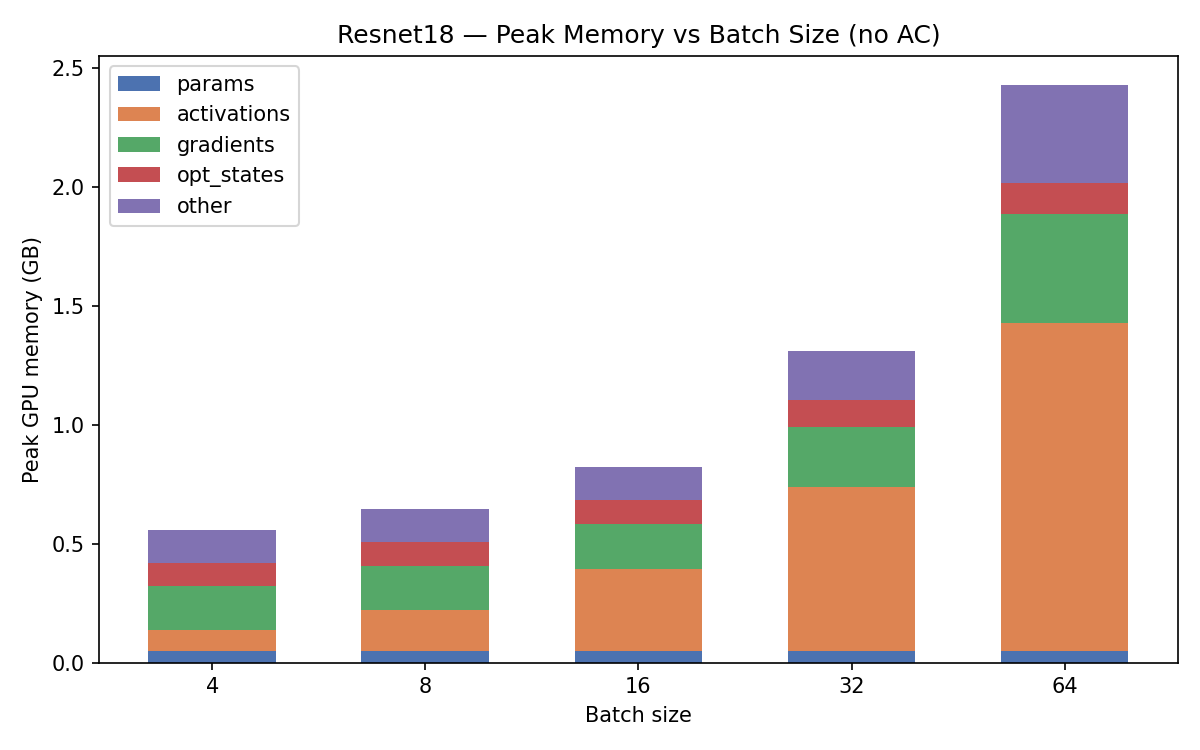
\includegraphics[width=\textwidth]{peak_memory_resnet18.png}
    \caption{ResNet18}
    \label{fig:mem_resnet18}
  \end{subfigure}
  \hfill
  \begin{subfigure}[b]{0.48\textwidth}
    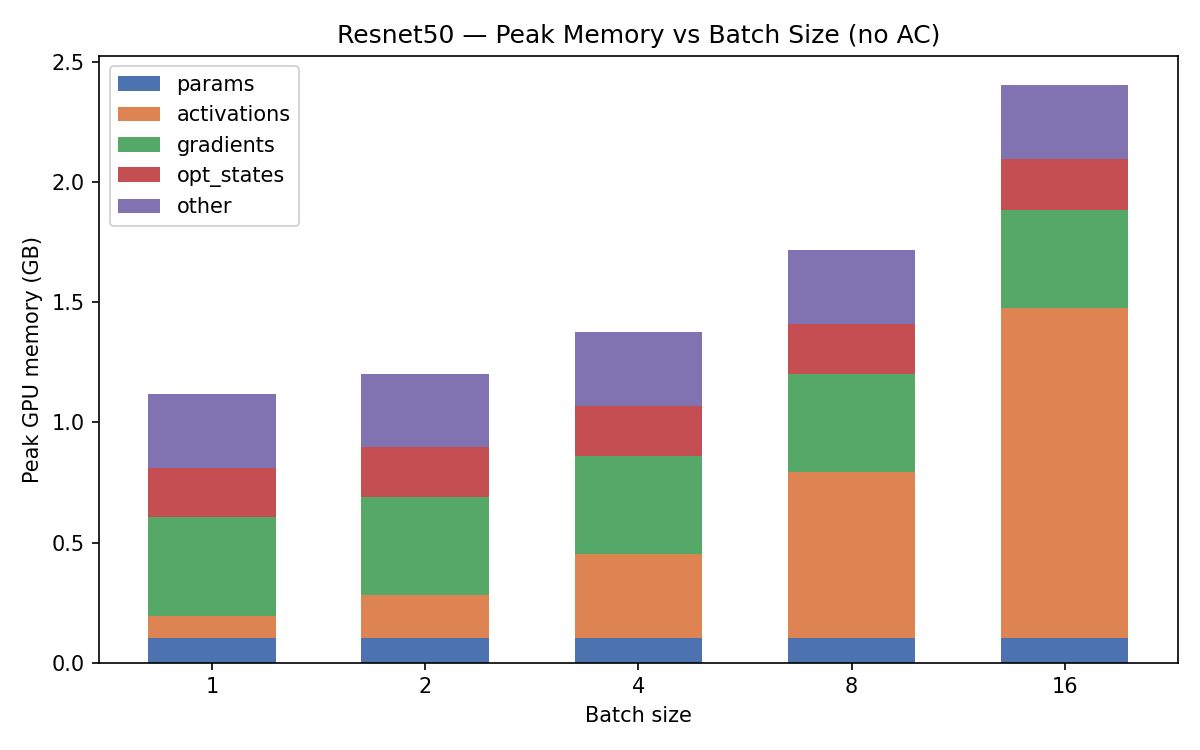
\includegraphics[width=\textwidth]{peak_memory_resnet50.png}
    \caption{ResNet50}
    \label{fig:mem_resnet50}
  \end{subfigure}
  \\[1em]
  \begin{subfigure}[b]{0.48\textwidth}
    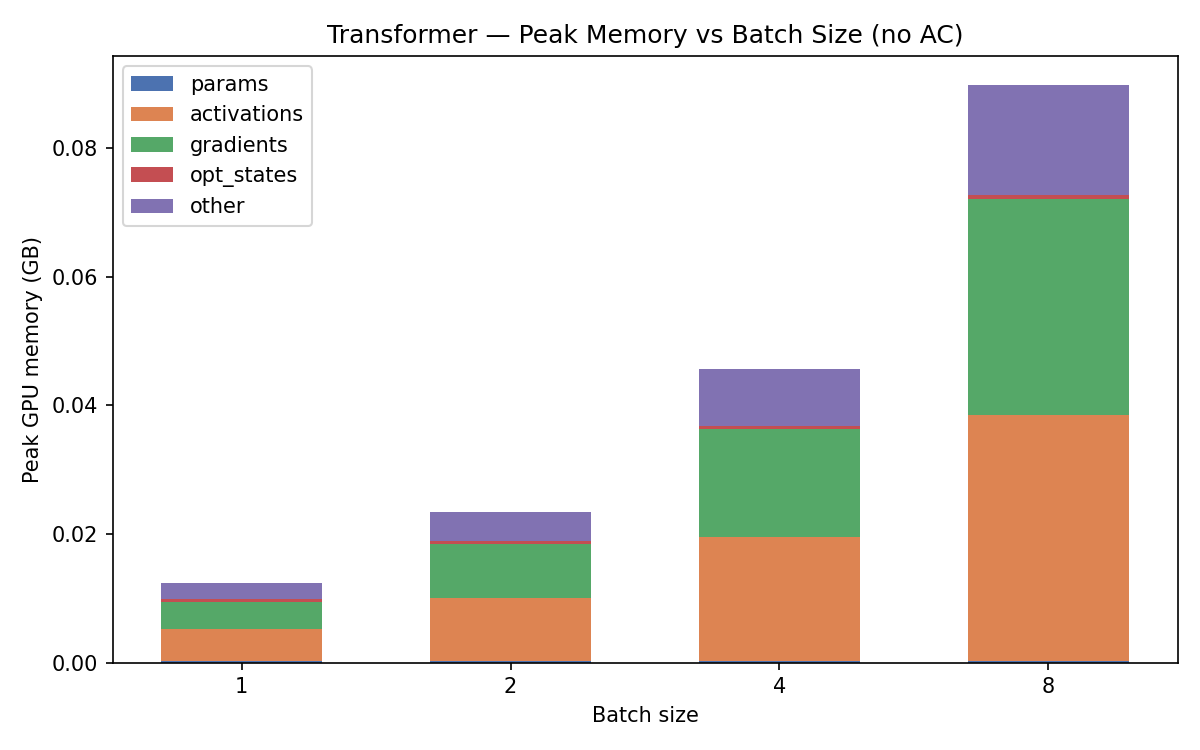
\includegraphics[width=\textwidth]{peak_memory_transformer.png}
    \caption{Transformer}
    \label{fig:mem_transformer}
  \end{subfigure}
  \caption{Peak GPU memory by category vs.\ batch size (no activation
           checkpointing). Activations scale linearly with batch size
           and account for the majority of memory in all three models.}
  \label{fig:memory}
\end{figure}

% ============================================================
\section{Challenges}
% ============================================================

\begin{itemize}[leftmargin=*]

  \item \textbf{Fused optimizer incompatibility with tracing.}
    The \texttt{fused=True} variant of Adam inspects \texttt{device.type}
    on its parameter tensors during \texttt{make\_fx} tracing, where
    tensors are fake and the device is \texttt{None}.
    This causes an \texttt{AttributeError} at trace time.
    Switching to \texttt{foreach=True} resolves the issue because that
    path decomposes into standard element-wise ATen ops that are fully
    compatible with fake-tensor tracing.

  \item \textbf{Memory attribution for multi-output ops.}
    Operations such as \texttt{\_foreach\_sqrt} return a list of tensors,
    each extracted by a child \texttt{getitem} node.
    The physical GPU allocation happens in the parent op, not in the
    \texttt{getitem} nodes, so attributing memory to each \texttt{getitem}
    would double-count.
    We record the full allocation at the parent and zero bytes at each
    \texttt{getitem}.

  \item \textbf{View operations and shared storage.}
    \texttt{view} and \texttt{reshape} nodes in the Transformer return
    tensors that share the underlying storage of their inputs.
    Our byte-size measurement reports the logical tensor size, not the
    incremental allocation, which causes the Transformer's activation
    memory estimate to be an overestimate of actual GPU usage.
    Correcting this requires tracking storage pointers across nodes, which
    we leave as a future improvement.

  \item \textbf{Graph scale.}
    The combined graph for ResNet50 contains over 4,000 nodes, making
    manual inspection impractical.
    All static analysis must be fully automated and produce correct
    results without per-model tuning.

  \item \textbf{Phase 2 interface.}
    The profiler must export a well-defined set of per-activation data
    (\texttt{size\_bytes}, \texttt{recompute\_time\_ms},
    \texttt{last\_fwd\_use}, \texttt{first\_bwd\_use}) for the Phase~2
    selection algorithm.
    We will finalize and test this interface as Phase~2 begins.

\end{itemize}

\end{document}
